\documentclass[./exercises.tex]{subfiles}
\begin{document}
\textit{\textbf{Tentamen 2021-06-22 } }\\

\begin{enumerate}
\item  $0.10$ kg is med temperaturen $0.0^o$C sänkes ned i $2.0$ kg vatten,
som har temperaturen $+80^o$C. Vilken blir blandningens sluttemperaturen?\\
Isens smältentalpi är 334 kJ/kg. Är processen reversibel?\\

Energi avgiven är lika med energi upptagen. Det varma vattnet avger energi som skall
smälta isen samt ge det smältvattnet en sluttemperatur som är blandningens temperatur
$T_f$
Givet:
\begin{flalign*}
m_1 &= 2.0\text{ kg}\\
m_2 &= 0.1\text{ kg}\\
T_1 &=80^o\text{C}\\
T_2 &=0.0^o\text{C}\\
c_{melt}&= 334 \text{ kJ/kg}\\
c_{H_20}&=4.19\text{ kJ/(kgK)}\\
\end{flalign*}
Energi avgiven är lika med energi upptagen
\begin{flalign*}
&|Q_{avgiven}|= |Q_{upptagen}|\\
&m_1c_{H_20}(T_2-T_f)=m_2c_{melt}+m_2c_{H_20}(T_f-T_2)\\
\end{flalign*}
Omfördelar termer
\begin{flalign*}
&m_1c_{H_20}T_2 -m_2c_{melt}=m_1c_{H_20}T_f+m_2c_{H_20}T_f\\
&T_f(m_1c_{H_20}+m_2c_{H_20})=m_1c_{H_20}T_2 -m_2c_{melt}\\
\end{flalign*}
Löser ut $T_f$
\begin{flalign*}
T_f&=\frac{m_1c_{H_20}T_2 -m_2c_{melt}}{m_1c_{H_20}+m_2c_{H_20}}\\
   &=\frac{2.0\cdot4.19\cdot 80 -0.1\cdot 334}{2.0\cdot 4.19 +0.1\cdot 4.19}\\
   &=72.394590294^o\text{C}
\end{flalign*}
vilket avrundas till en värdesiffra i decimalen.\\
Blandningens temperatur blir $72.4^o$C.\\


\vfill\null
\clearpage
\columnbreak
\newpage

\item I en trycktank finns $2m^3$ luft, temperatur $+20^o$C och tryck 100 kPa.\\
Med hjälp av en kompressor, som arbetar isotermiskt, ska trycket i tanken höjas 10 gånger.\\
Kompressorn suger in 20 liter luft (temperatur $+20^o$C och tryck 100 kPa) per sekund.\\
Hur länge måste kompressorn arbeta innan trycket i tanken har \oe kat 10 gånger?\\

Givet
\begin{flalign*}
V &=2m^3\\
T&=+20^oC = 293^oK\\
p_1 &= 100kPa\\
p_2 &= 10\cdot p_1\\
\dot{V} &= 20 dm^3/s = 0.02m^3/s\\
\end{flalign*}
Kompressorn tillför massa $m_{tillf}$ till tanken.
Innan kompressorn startar så finns luftmassa $m_1$ i tanken
\begin{flalign*}
m_1 &=\frac{p_1\cdot V}{R\cdot T}
\end{flalign*}
När trycket har uppnåtts så  kommer
massan i tanken vara $m_2$ sådant att
\begin{flalign*}
m_2 &=\frac{p_2V}{RT}\\
    &=\frac{10p_1 V}{RT}\\
\end{flalign*}
Den massa som måste tillföras är $m_{tillf}=m_2-m_1$.
\begin{flalign*}
m_{tillf}&=m_2-m_1\\
        &=\frac{10p_1V}{RT}-\frac{p_1 V}{RT}\\
        &=\frac{9p_1V}{RT}\\
\end{flalign*}
Massflödet $\dot{m}$ som kompressorn åstadkommer är
\begin{flalign*}
\dot{m} &=\rho\dot{V}
\end{flalign*}
d\ae r $\rho$ är
\begin{flalign*}
\rho&=\frac{m_1}{V}=\frac{p_1}{RT}
\end{flalign*}
Så för att åstadkomma masstillskottet $m_{tillf}$ krävs tiden $\Delta t$
\begin{flalign*}
\dot{m}\Delta t &=m_{tillf}\\
                &=\frac{9p_1V}{RT}\\
\end{flalign*}
Substituerar $\rho\dot{V}$ for $\dot{m}$ för att sedan
ersätta $\rho$ med dess uttryck från den allmänna gaslagen
\begin{flalign*}
\rho\dot{V}\Delta t&=\frac{9p_1V}{RT}\\
\frac{p_1}{RT}\dot{V}\Delta t&=\frac{9p_1V}{RT}\\
\end{flalign*}
$p_1$ och $RT$ försvinner från båda sidor
\begin{flalign*}
\Delta t&=\frac{9p_1V}{RT}\frac{RT}{p_1\dot{V}}\\
        &=\frac{9V}{\dot{V}}\\
        &=\frac{9\cdot 2}{0.02}=900s\\
\end{flalign*}

Tiden som behövs för att kompressorn ska öka trycket 10 ggr
är således relaterad till att öka luftmassan i den slutna
cylindern från $m_1$ till $m_2$ och är 900 sekunder med
flödet 20 liter per sekund.\\


\vfill\null
\clearpage
\columnbreak
\newpage

\item En behållare har volymeb $15.0$l och innehåller $1.00$kg syrgas $(\kappa = 1.40)$,
som har temperaturen $+27^o$C. Gasen får expandera isotermiskt till slutvolymen
$45.0$l varvid trycket blir $p_{iost}$.\\
Om gasen istället expanderat adiabatiskt till slutvolymen så hade trycket blivit $p_{adi}$.\\
a.) Beräkna kvoten $p_{isot}/p_{adi}$.\\
b.) Vilken sluttemperatur har gasen i det adiabatiska fallet\\

Givet
\begin{flalign*}
p_1 &=?\\
m &= 1kg\\
T_1 &=27^oC = 300^oK\\
V_1 &=15.0l=0.015m^3\\
V_2 &=45.0l=0.045m^3\\
\end{flalign*}
a.)\\
När en gas genomgår en isotermisk process gäller följande mellan start och sluttillståndet
\begin{flalign*}
T_1&=\frac{p_1V_1}{mR}=T_2=\frac{p_2V_2}{mR}\\
p_1V_1 &=p_2V_2
\end{flalign*}
Således är det trycket $p_2$ efter den isotermiska expanisionen
\begin{flalign*}
p_2 &=p_1\frac{V_1}{V_2}\\
   &=p_1\frac{15}{45}=\frac{p_1}{3}\\
\end{flalign*}
För att hitta relationen för hur en adiabatisk process
beter sig utgår vi från definitionen av entropi
\begin{flalign*}
s_2-s_1 &=\int_1^2\Big(\frac{dq}{T}\Big)_{rev}\\
        &=\int_1^2\frac{1}{T}(du+p\cdot dv)\\
		&=\int_1^2\frac{1}{T}(c_vdT+\frac{R\cdot T}{V}\cdot dv)\\
        &=\int_1^2c_v\frac{dT}{T}+R\cdot \frac{dv}{v}\\
\end{flalign*}
Vi skriver $\bar{c_v}$ såsom ett konstant medelvärde mellan integrations gränserna
och antar att $R$ är konstant mellan integrations gränserna också
\begin{flalign*}
s_2-s_1 &=c_v\int_1^2\frac{dT}{T}+R\int_1^2\frac{dv}{v}\\
        &=c_v\cdot ln\frac{T_2}{T_1} + R\cdot ln\frac{v_2}{v_1}&(1)\\
\end{flalign*}
Då  $s_2-s_1 = 0$ under en isentrop process så  gäller att
\begin{flalign*}
c_v\cdot ln\frac{T_2}{T_1} + R\cdot ln\frac{v_2}{v_1} =0\\
\end{flalign*}
och då gäller
\begin{flalign*}
c_v\cdot ln\frac{T_2}{T_1} &=- R\cdot ln\frac{v_2}{v_1}\\
ln\frac{T_2}{T_1} &=- \frac{R}{c_v}\cdot ln\frac{v_2}{v_1}\\
                  &=\frac{R}{c_v}\cdot ln\frac{v_1}{v_2}\\
                  &=\frac{c_p-c_v}{c_v}\cdot ln\frac{v_1}{v_2}\\
				  &=(\kappa -1)\cdot ln\frac{v_1}{v_2}\\
                  &=ln\Big(\frac{v_1}{v_2}\Big)^{\kappa -1}
\end{flalign*}
vilket vi kan skriva utan per massenhet notationen såsom
\begin{flalign*}
\frac{T_2}{T_1} &=\Big(\frac{V_1}{V_2}\Big)^{\kappa -1}
\end{flalign*}
Eftersom kvoterna är konstant så måste även produkterna
$T_1V_1^{\kappa -1}$ och $T_2V_2^{\kappa -1}$ vara konstanter och lika.\\
Vi kan således skriva relationen
\begin{flalign*}
T\cdot V^{\kappa-1} &=\text{ konstant}
\end{flalign*}
Eftersom allmänna gaslagen ger att
\begin{flalign*}
p_2\cdot v_2 &=m\cdot R\cdot T_2\\
p_1\cdot v_1 &=m\cdot R\cdot T_1 \text{ så}\\
\frac{T_2}{T_1}&=\frac{p_2\cdot v_2 }{p_1\cdot v_1}
\end{flalign*}
så ekvation $(1)$ kan också skrivas
\begin{flalign*}
s_2-s_1  &=c_v\cdot ln\frac{T_2}{T_1} + R\cdot ln\frac{v_2}{V_1}\\
         &=c_v\cdot ln\frac{p_2\cdot v_2 }{p_1\cdot v_1} + R\cdot ln\frac{v_2}{v_1}\\
		 &=c_v\cdot ln\frac{p_2 }{p_1}+c_v\cdot ln\frac{v_2 }{v_1} + (c_p-c_v)\cdot ln\frac{v_2}{v_1}\\
		 &=c_v\cdot ln\frac{p_2 }{p_1}+ c_p\cdot ln\frac{v_2}{v_1}\\
\end{flalign*}
Om vi då sätter $s_2-s_1 = 0$ så får vi
\begin{flalign*}
0&=c_v\cdot ln\frac{p_2 }{p_1}+ c_p\cdot ln\frac{v_2}{v_1}\\
\end{flalign*}
och då får vi
\begin{flalign*}
c_v\cdot ln\frac{p_2 }{p_1}&=- c_p\cdot ln\frac{v_2}{v_1}\\
ln\frac{p_2 }{p_1}&=- \frac{c_p}{c_v}\cdot ln\frac{v_2}{v_1}\\
                  &=\frac{c_p}{c_v}\cdot ln\frac{v_1}{v_2}\\
                  &=\kappa\cdot ln\frac{v_1}{v_2}\\
                  &=ln\Big(\frac{v_1}{v_2}\Big)^\kappa
\end{flalign*}
eller
\begin{flalign*}
\frac{p_2 }{p_1}&=\Big(\frac{v_1}{v_2}\Big)^\kappa\\
\end{flalign*}
vilket också kan skrivas utan per massenhet notation såsom
\begin{flalign*}
p_1\cdot V_1^\kappa &=p_2\cdot V_2^\kappa\\
\end{flalign*}
vilket är en den andra formeln i formelsamlingen som beskriver
hur en adiabatisk process förhåller sig från starttilsttånd till sluttillstånd.\\

Så trycket $p_{adi}$ efter den adiabatiska expansionen är
\begin{flalign*}
p_1\cdot V_1^\kappa &=p_2\cdot V_2^\kappa\\
p_{adi} &=p_1\Big(\frac{V_1}{V_2}\Big)^\kappa\\
        &=p_1\Big(\frac{15}{45}\Big)^{1.4}\\
        &=p_1\Big(\frac{1}{3}\Big)^{1.4}\\
\end{flalign*}
Kvoten $p_{isot}/p_{adi}$ blir då
\begin{flalign*}
\frac{p_{isot}}{p_{adi}} &= \frac{\frac{p_1}{3}}{p_1\Big(\frac{1}{3}\Big)^{1.4}}\\
                       &=\frac{3^{1.4}}{3}=3^{0.4}=1.55\\
\end{flalign*}

b.)\\
Sluttemperaturen i det adiabatiska fallet förhåller sig såsom
\begin{flalign*}
T_1\cdot V_1^{\kappa-1} &=T_2\cdot V_2^{\kappa-1}
\end{flalign*}
vilket ger att
\begin{flalign*}
T_2&=T_1\Big(\frac{V_1}{V_2}\Big)^{\kappa-1}\\
   &=300\Big(\frac{15}{45}\Big)^{0.4}\\
   &=300\Big(\frac{1}{3}\Big)^{0.4}= 193.32^oK=-79.7^oC\\
\end{flalign*}


\vfill\null
\clearpage
\columnbreak
\newpage

\item 10 liter torr luft med temperaturen $+20^o$C har trycket $1.0$ bar $= 100$ kPa.
 Luften komprimeras vid konstant tryck så att dess volym halveras.
 Behöver värme tillföras eller bortföras? Hur många Joule?
 Hur mycket ändras luftens inre energi?
 Data för luft tas ifrån sid 16 i formelsamlingen.\\
 
Givet
\begin{flalign*}
V&=10l=0.01m^3\\
p_1&=1bar=10^5Pa\\
T_1 &=+20^oC = 293^oK\\
V_2 &=5l = 0.005m^3
\end{flalign*}
Eftersom trycket inte ändras då kompressionen sker så måste värme
hela tiden bortföras.
För en isobar kompression så måste värmemängden $Q_{12}$ bortföras enligt
\begin{flalign*}
Q_{12} &= m\bar{c}_p(T_2-T_1)
\end{flalign*}
där $T_2$ och $T_1$ förhåller sig under en isobar process såsom
\begin{flalign*}
\frac{V_1}{T_1}&=\frac{V_2}{T_2}\\
\end{flalign*}
vilket betyder att $T_2$ fås såsom
\begin{flalign*}
T_2&=T_1 \frac {V_2}{V_1}\\
   &=293\frac {0.005}{0.01}\\
   &=146.5^oK=-126.5^oC
\end{flalign*}
Den värmemängd som måste bortföras kan nu beräknas.
Formelsamlingens lägsta temperatur för vilket $c_p$ är angivet är för
$-100^o$C där $c_p = 1.012$ kJ/(kg$\cdot$K) och massan $m$ beräknas
med allmänna gaslagen till och $R=287$ J/(kg$\cdot$K)
\begin{flalign*}
m&=\frac{p_1\cdot V_1}{R\cdot T_1}\\
  &=\frac{10^5\cdot 0.01}{287\cdot 293}\\
  &=0.011891879 kg
\end{flalign*}
Insättning ger
\begin{flalign*}
Q_{12} &= m\bar{c}_p(T_1/2-T_1)\\
       &= 0.011891879\cdot 1012(-146.5)\\
       &=-1763.066196782J \approx -1763J
\end{flalign*}
Ändringen i inre energi kan beräknas på två sätt.
Antingen använder vi $c_p-c_v = R$ vilket ger $c_v=c_p-R$
och räknar
\begin{flalign*}
U_{12} &= m\bar{c}_v(T_1/2-T_1)\\
       &= 0.011891879\cdot (1012-287)(-146.5)\\
       &=-1263.066198287J \approx -1263J
\end{flalign*}
or we use
\begin{flalign*}
Q_1 &= U_{12}+W_12\\
U_{12}&=Q_1 -W_12\\
      &=-1763.066196782J -p_1(V_2-V_1)\\
      &=-1763.066196782J -10^5(0.005-0.01)\\
      &=-1763.066196782J +500 \approx -1263J\\
\end{flalign*}


\vfill\null
\clearpage
\columnbreak
\newpage

\item Temperaturen i ett kylskåp ska vara $0.0^o$C, och rummet i vilket kylskåpet är placerat
har temperaturen $+20^o$C. Hur stor effekt måste vi tillföra kylmaskinen,
om denna är en ideal carnotmaskin och det per dygn läcker in $10^7$ J värme i kylskåpet?\\

Givet
\begin{flalign*}
T_1 &= 20^oC=293^oK\\
T_2 &= 0.0^oC = 273^oK\\
\dot{Q}_{tillf} &= 10^7 J/dygn = 10^7/(24\cdot 3600) W\\
\end{flalign*}
Sökt är $\dot{W}_t$ det tekniska arbetet per tidsenhet som måste tillföras kylprocessen.

\begin{figure}[h]
\centering
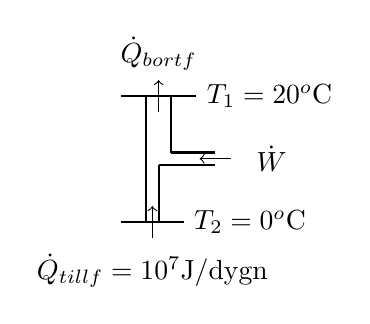
\begin{tikzpicture}[ scale=.4,baseline={(0,0)}]
%\draw upper 

\draw [thick] (1,0) -- (3,0) node[right]{    $T_2=0^o$C};%Basen för Q tillförd

\draw [thick] (1,4) -- (3.4,4) node[right]{    $T_1=20^o$C};%Basen för Q bortförd
\draw [thick] (1.8,0) -- (1.8,4); %Vänster kanalvägg
\draw [thick] (2.2,0) -- (2.2,1.8); %Höger kanalvägg
\draw [thick] (2.2,1.8)--(4,1.8); %w nedre kanalvägg
\draw [thick] (4,2.2)-- (2.6,2.2); %w övre kanalvägg
\draw [thick] (2.6,2.2)-- (2.6,4); %höger kanalvägg upp till bas

\draw[->] (2,-0.5) -- (2,0.5);
\node[below] (a) at (2,-0.7){$\dot{Q}_{tillf}=10^7$J/dygn};

\draw[->] (4.5,2) -- (3.5,2);
\node[right] (b) at (5,2){$\dot{W}$};

\draw[->](2.2,3.5)--(2.2,4.5) node[above]{$\dot{Q}_{bortf}$};

\end{tikzpicture}
\end{figure}

Enligt formelsamlingen gäller att för köldfaktorn $\epsilon$ för en kylmaskin
är
\begin{flalign*}
\epsilon &=\left|\frac{Q_{tillf}}{W_t}\right|
\end{flalign*}
för en Carnot kylmaskin så gäller att kretsprocessen ser ut som följer
\begin{figure}[h]
\centering
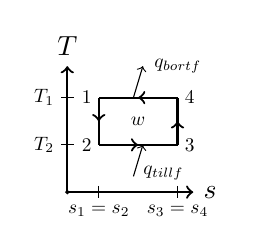
\begin{tikzpicture}[scale=.4,baseline={(0,0)}]
%\begin{tikzpicture}[show background rectangle, scale=.5]

%\draw (0,0) grid (4,4);
% x-axis
\draw [thick,->] (0,0) -- (4,0) node[right]{$s$};
% y-axis
\draw [thick,->] (0,0) -- (0,4) node[above]{$T$};
% x-axis label
%\node at (-0.3,4){$T$};
% y-axis label
%\node at (4,-0.3){$s$};
%origin point
\draw [color=black,fill=black] (0,0) circle (0.05);

\draw[thick](1,1.5)--(3.5,1.5)node[scale=0.7, right]{3};
\draw[thick,->](1,1.5)--(2.25,1.5);

\draw[thick](3.5,1.5)--(3.5,3)node[scale=0.7,right]{4};
\draw[thick,->](3.5,1.5)--(3.5,2.25);

\draw[thick](3.5,3)--(1,3)node[scale=0.7, left]{1};
\draw[thick,->](3.5,3)--(2.25,3);

\draw[thick](1,3)--(1,1.5)node[scale=0.7, left]{2};
\draw[thick,->](1,3)--(1,2.25);

\draw[->](2.1,0.5)--(2.4,1.5);%q_tillf pil
\draw[->](2.1,3)--(2.4,4);%q_bortf pil

\node[right,scale=0.7] (a) at (2.2,0.6){$q_{tillf}$};
\node[scale=0.7] (c) at (2.25,2.25){$w$};
\node[right,scale=0.7] (d) at (2.55,4.0){$q_{bortf}$};

\draw (1,0.2)--(1,-0.2) node[below,scale=0.7]{$s_1=s_2$};
\draw (3.5,0.2)--(3.5,-0.2) node[below,scale=0.7]{$s_3=s_4$};

\draw(0.2,3)--(-0.2,3) node[left,scale=0.7]{$T_1$};
\draw(0.2,1.5)--(-0.2,1.5) node[left,scale=0.7]{$T_2$};

\end{tikzpicture}
\end{figure}

Vi kan nu teckna köldfaktorn för carnot maskinen därför
att $Q_{tillf}$ är arean under kurvan från $2\rightarrow 3$
och $W_t$ är den inneslutna arean.
\begin{flalign*}
\epsilon &=\left|\frac{Q_{tillf}}{W_t}\right|\\
\epsilon_c&=\frac{T_2(s_3-s_2)}{T_1(s_3-s_2)-T_2(s_3-s_2)}\\
\end{flalign*}
Observera att det känns lite ointuivt att sätta in den låga temperaturen i täljaren
då $Q_{tillf}$ är p.g.a. rumstemperaturen, men det är helt korrekt.
\begin{flalign*}
\epsilon_c&=\frac{T_2}{T_1-T_2}\\
         &=\frac{273}{293-273}=13.63\\
\end{flalign*}
Denna ködfaktorkvot kan användas för att få fram $\dot{W}_t$
därför att kvoten mellan $\dot{Q}_{tillf}$ och $\dot{W}_t$ måste hela
tiden vara konstant och lika med köldfaktorn som är uträknad för en cykel.
\begin{flalign*}
\epsilon_c&=13.63=\frac{\dot{Q}_{tillf}}{\dot{W}_t}\iff\\
\dot{W}_t &=\frac{\dot{Q}_{tillf}}{13.63}\\
          &=\frac{10^7}{24\cdot 3600\cdot 13.63} \\
		  &=8.491617076W\approx 8.5 W
\end{flalign*}


\vfill\null
\clearpage
\columnbreak
\newpage


\item En ideal gas befinner sig i ett tillstånd  $(p_1,V_1,T_1)$.
Gasen först via en isoterm process till $(p_2,V_2,T_2)$ där $V_2 = 2V_1$,
följt av en adiabatisk expansion till $(p_3,V_3,T_3)$ där $V_3 = 3V_1$.\\
Därefter följer en isobar och en isokor process, vilka för systemet tillbaka
till begynnelsetillståndet.
Alla processer är reversibla.
Rita ett $p/V$-diagram och ett $T/s$-diagram över kretsprocessen.
Beräkna entropiändringarna för varje delprocess och
avsluta sedan med att beräkna summan av alla entropiändringar för ett varv.\\

När man ska rita en kretsprocess i ett $T/s$-diagram så får man komma ihåg
att alla processer utom den polytropiska med $n < \kappa$ går i
syd-väst till/från nord-ost där alltså endast den nämda polytropa
processen går mellan nord-väst och syd-ost.

För den isoterma processen har vi
\begin{flalign*}
p_1V_1 &= p_2V_2 =p_22V_1\iff\\
p_2 &= p_1/2\\
T_1 &=T_2
\end{flalign*}
Sammanfattningsvis så har vi efter isotermen
\begin{flalign*}
p_2 &= p_1/2\\
V_2 =2V_1 \\
T_1 &=T_2\\
\end{flalign*}
därefter följer den adiabatiska expansionen
\begin{flalign*}
p_2V_2^\kappa &= p_3V_3^\kappa =p_3(3V_1)^\kappa\\
p_2(2V_1)^\kappa &= p_3V_3^\kappa =p_3(3V_1)^\kappa\iff\\
p_3&=p_2\Big(\frac{2}{3}\Big)^\kappa\\
    &=\frac{p_1}{2}\Big(\frac{2}{3}\Big)^\kappa\\
\end{flalign*}
där $T_3$ och $T_2$ förhåller sig enligt
\begin{flalign*}
\frac{T_3}{T_2}&=\Big(\frac{V_2}{V_3}\Big)^{\kappa-1}
\end{flalign*}
vilket ger
\begin{flalign*}
T_3&=T_2\Big(\frac{2V_1}{3V_1}\Big)^{\kappa-1}\\
   &=T_1\Big(\frac{2}{3}\Big)^{\kappa-1}\\
\end{flalign*}
Sammanfattnignsvis så har vi efter adiabaten
\begin{flalign*}
p_3&=\frac{p_1}{2}\Big(\frac{2}{3}\Big)^\kappa\\
V_3&=3V_1\\
T_3&=T_1\Big(\frac{2}{3}\Big)^{\kappa-1}\\
\end{flalign*}
Vidare följer en isobar process där vi har att
trycket är konstant
\begin{flalign*}
p_4 &=p_3 = \frac{p_1}{2}\Big(\frac{2}{3}\Big)^\kappa\\
\end{flalign*}
Volymen och temperaturen förhåller sig enligt
\begin{flalign*}
\frac{V_4}{T_4}&= \frac{V_3}{T_3}
\end{flalign*}
men här verkar jag inte kunna lösa ut $V_4$ och $T_4$
Däremot så vet vi att processen går som en isokor till $(p_1,V_1,T_1)$
Men om $V_4$ till $V_1$ är en iskor process så är ju $V_4=V_1$ 
så 
\begin{flalign*}
\frac{V_4}{T_4}&= \frac{V_3}{T_3}\\
\frac{V_1}{T_4}&= \frac{3V_1}{T_3}\iff\\
T_4 &= T_3/3
\end{flalign*}
Sammanfattningsvis så har vi efter den isobara processen
\begin{flalign*}
p_4 &=\frac{p_1}{2}\Big(\frac{2}{3}\Big)^\kappa\\
V_4 &=V_1\\
T_4 &= \frac{1}{3}T_1\Big(\frac{2}{3}\Big)^{\kappa-1}\\
\end{flalign*}

Samtliga sammanfattningar
Från $(p_1,V_1, T_1)$ och isoterm till
\begin{flalign*}
p_2 &= p_1/2\\
V_2 =2V_1 \\
T_1 &=T_2\\
\end{flalign*}
och därefter adiabat till
\begin{flalign*}
p_3&=\frac{p_1}{2}\Big(\frac{2}{3}\Big)^\kappa\\
V_3&=3V_1\\
T_3&=T_1\Big(\frac{2}{3}\Big)^{\kappa-1}\\
\end{flalign*}
och därefter isobar till
\begin{flalign*}
p_4 &=\frac{p_1}{2}\Big(\frac{2}{3}\Big)^\kappa\\
V_4 &=V_1\\
T_4 &= \frac{1}{3}T_1\Big(\frac{2}{3}\Big)^{\kappa-1}\\
\end{flalign*}
och därefter isokor till  $(p_1,V_1, T_1)$.
Entropiändringen för isotermen är
\begin{flalign*}
s_2-s_1 &= R\cdot ln\frac{V_2}{V_1}=R\cdot ln\frac{p_1}{p_2}\\
         &=R\cdot ln\frac{2V_1}{V_1}=R\cdot ln\frac{p_1}{p_1/2}\\
         &=R\cdot ln 2
\end{flalign*}
Entropiändringen för adiabaten är 0.
Entropiändringen för isobaren är
\begin{flalign*}
s_4-s_3 &=\bar{c}_p ln \frac {T_4}{T_3}=\bar{c}_p ln \frac {V_4}{V_3}\\
        &=\bar{c}_p ln \frac { T_3/3}{T_3}=\bar{c}_p ln \frac {V_1}{3V_1}\\
		&=\bar{c}_p ln \frac {1}{3}\\
\end{flalign*}
och slutligen entropiändringen för isokoren
\begin{flalign*}
s_1-s_4 &= \bar{c}_vln\frac{T_1}{T_4}=\bar{c}_vln\frac{p_1}{p_4}\\
        &= \bar{c}_vln\frac{T_1}{ \frac{1}{3}T_1\Big(\frac{2}{3}\Big)^{\kappa-1}}=\bar{c}_vln\frac{p_1}{\frac{p_1}{2}\Big(\frac{2}{3}\Big)^\kappa}\\
		&=\bar{c}_vln\frac{2}{\Big(\frac{2}{3}\Big)^\kappa}\\
\end{flalign*}

Summera dessa:
\begin{flalign*}
s_2-s_1 &=R\cdot ln 2\\
s_4-s_3 &=\bar{c}_p ln \frac {1}{3}=-\bar{c}_p ln 3\\
s_1-s_4 &=\bar{c}_vln\frac{2}{\Big(\frac{2}{3}\Big)^\kappa}\\
\end{flalign*}
Först måste vi slå isär termen $s_1-s_4$
\begin{flalign*}
s_1-s_4&=\bar{c}_vln\frac{2}{\Big(\frac{2}{3}\Big)^\kappa}\\
&=\bar{c}_vln 2-\bar{c}_vln\Big(\frac{2}{3}\Big)^\kappa\\
&=\bar{c}_vln 2-\bar{c}_v\kappa ln 2 + \bar{c}_v\kappa ln 3\\
&=\bar{c}_vln 2-\bar{c}_p ln 2 + \bar{c}_p ln 3\\
\end{flalign*}
Nu har vi ett bättre uttryck för $s_1-s_4$ och kan summera 
samtliga termer på ett mer transparent vis
\begin{flalign*}
&R\cdot ln 2 -\bar{c}_p ln 3\\
&+\bar{c}_vln 2-\bar{c}_p ln 2 + \bar{c}_p ln 3\\
&=R\cdot ln 2-(\bar{c}_p-\bar{c}_v)ln 2\\
&+\bar{c}_p ln 3-\bar{c}_p ln 3=0
\end{flalign*}
där det faktum att $R= c_p-c_v$ har utnyttjats.



\vfill\null
\clearpage
\columnbreak
\newpage


\item Vattenånga med trycket 20 bar och \\
$x=95\%$ strömmar genom en strypventil.
Efter ventilen är trycket 5.0 bar. Vid passagen ändras inte ångans entalpi.
Däremot ökar ångans entropi. Beräkna hur stor entropiökningen är.\\

Här ska man ha en $T/s$ graf som visar att för specifika ånghalten $x=1$ så går temperaturen som funktion
av entropin som en symmetrisk trubbig avrundad bergstopp där streckade linjer för specifika ånghalten går som
rinnande vatten ådrår från toppen som är den kritiska punkten. Vid den kritiskpunkten
finns ingen klar övergång från vätska till ånga, skilje ytan mellan ångfaserna blir osynlig.
Ytan som innesluts av ``berget'' är tillståndet för den fuktiga ångan. Till vänster
om berget finns den mättade vätskan och till höger finns torr mättad ånga.
Trycket $p$ löper som horisontella linjer som skär berget och först vid den högra
gränsen så sticket kurvorna för respektive $p$-värde uppåt exponentiellt.
Ovanför den kritiska punkten finns både vätska och överhettad ånga men där skiljelinjen
$p>p_k$.

Den specifika volymen för fuktig ånga beräknas med formeln
\begin{flalign*}
v_f &=(1-x)\cdot v'+x\cdot v''
\end{flalign*}
där $v'$ är den specifika volymen för kokande vätska vid rådande tryck
och $v''$ är den specifika volymen för mättad ånga vid rådande tryck.
På samma sätt har vi
\begin{flalign*}
i_f &=(1-x)\cdot i'+x\cdot i''
\end{flalign*}
där $i'$ är entalpin för kokande vätska vid rådande tryck och $i''$ är entalpin
för mättad ånga vid rådande tryck.
och för entropin
\begin{flalign*}
s_f &=(1-x)\cdot s'+x\cdot s''
\end{flalign*}

Vidare har vi att luftens ångkvot dvs. den specifika ånghalten $x$ kan beräknas
som funktion av relativa ångtrycket (realtiva fuktigheten) $\varphi$ enligt
\begin{flalign*}
x&=0.621\frac{\varphi\cdot p_{H_20}''}{p-p_{H_20}''}
\end{flalign*}
och den fuktiga luftens entalpi $i$ kan också fås enligt
\begin{flalign*}
i &=c_{pL}\cdot t +x(r_o + c_{p_{H_20}}\cdot t) &(1)
\end{flalign*}
där \\
$t=$ lufttemperatur\\
$c_{pL}=$ luftens specifika värme vid konstant tryck\\
$r_o=$ vattnets ångbildningsvärme vid $0^o$C\\
$x=$ luftens ångkvot.
Med insatta värden erhålles, vid atmosfärstryck $=101.3$kPa.
\begin{flalign*}
i &\approx t +x\cdot(2500+ 1.86\cdot t) kJ/kg torrluft 
\end{flalign*}
Är fuktig ånga samma sak som fuktig luft? Jo, så måste det vara därför
att storheterna i ångtabeller ges i enheten per kg tott luft.

För att lösa ovan problem\\
Givet
\begin{flalign*}
p_1 &= 20 bar\\
x_1 &=0.95\\
p_2 &= 5bar\\
\end{flalign*}

Vi beräknar först entalpin men vi kan inte använd $(1)$ därför att
vi inte känner samtliga ingående delar så vi måste använda
ångtabeller
\begin{flalign*}
i_f &=(1-x)\cdot i'+x\cdot i''\\
i_f(p_1,x_1)&=(1-0.95)\cdot 908.60\\
           &+0.95\cdot 2798.96\\
                   &=2704.442 \text{kJ/kg torrluft}\\
\end{flalign*}
Entropin hos den fuktiga ångan är
\begin{flalign*}
s_f &=(1-x)\cdot s'+x\cdot s''\\
s_{f1}(p_1,x_1) &=(1-0.95)\cdot 2.4469\\
                &+0.95\cdot 6.3403\\
                    &=6.14563 \text{kJ/K*kg torrluft}\\
\end{flalign*}
För att ta reda på vad den nya specifika ånghalten är den s.k. ångkvoten
så måste vi identifiera denna utifrån det faktum att entalpin inte har
ändrats.
\begin{flalign*}
i_f &=(1-x_2)\cdot i'+x_2\cdot i''\\
\frac{i_f-i'}{i''-i'} & = x_2\\
\frac{2704.442-640.16}{2748.79-640.16} &= x_2\iff\\
x_2&=0.978968335\\
\end{flalign*}
Om vi nu använder denna nya specifika ånghalt $x_2$ så fås
avseende den nya entropin
\begin{flalign*}
s_f &=(1-x)\cdot s'+x\cdot s''\\
s_{f2}(p_2,x_2) &=(1-0.978968335)\cdot 1.8604\\
                 &+0.978968335\cdot 6.8219\\
                 &=6.717551394\text{ kJ/K*kg torrluft}\\
\end{flalign*}
Entropiökningen är
\begin{flalign*}
s_{f2}-s_{f1}&=6.717551394-6.14563\\
&=0.571921394\approx 0.57\text{ kJ/K*kg torrluft}
\end{flalign*}

\vfill\null
\clearpage
\columnbreak
\newpage

\item Luft med temperaturen $+10^o$C och relativa fuktigheten $\varphi=0,40$
värms till $+32,5^o$C. Hur stor blir nu $\varphi$?\\
Hur mycket ånga måste du tillsätta, vid denna temperatur,
för att komma tillbaks till $\varphi = 0.40$?\\
Ta data ifrån bifogat Mollier-diagram.
Rita en förenklad skiss över Mollier-diagrammet där du markerar alla
intressanta tillstånd och de värden du avläser i det bifogade Mollier-diagrammet.
Lämna in din skiss tillsammans med dina lösningar.

\begin{figure}[H]
  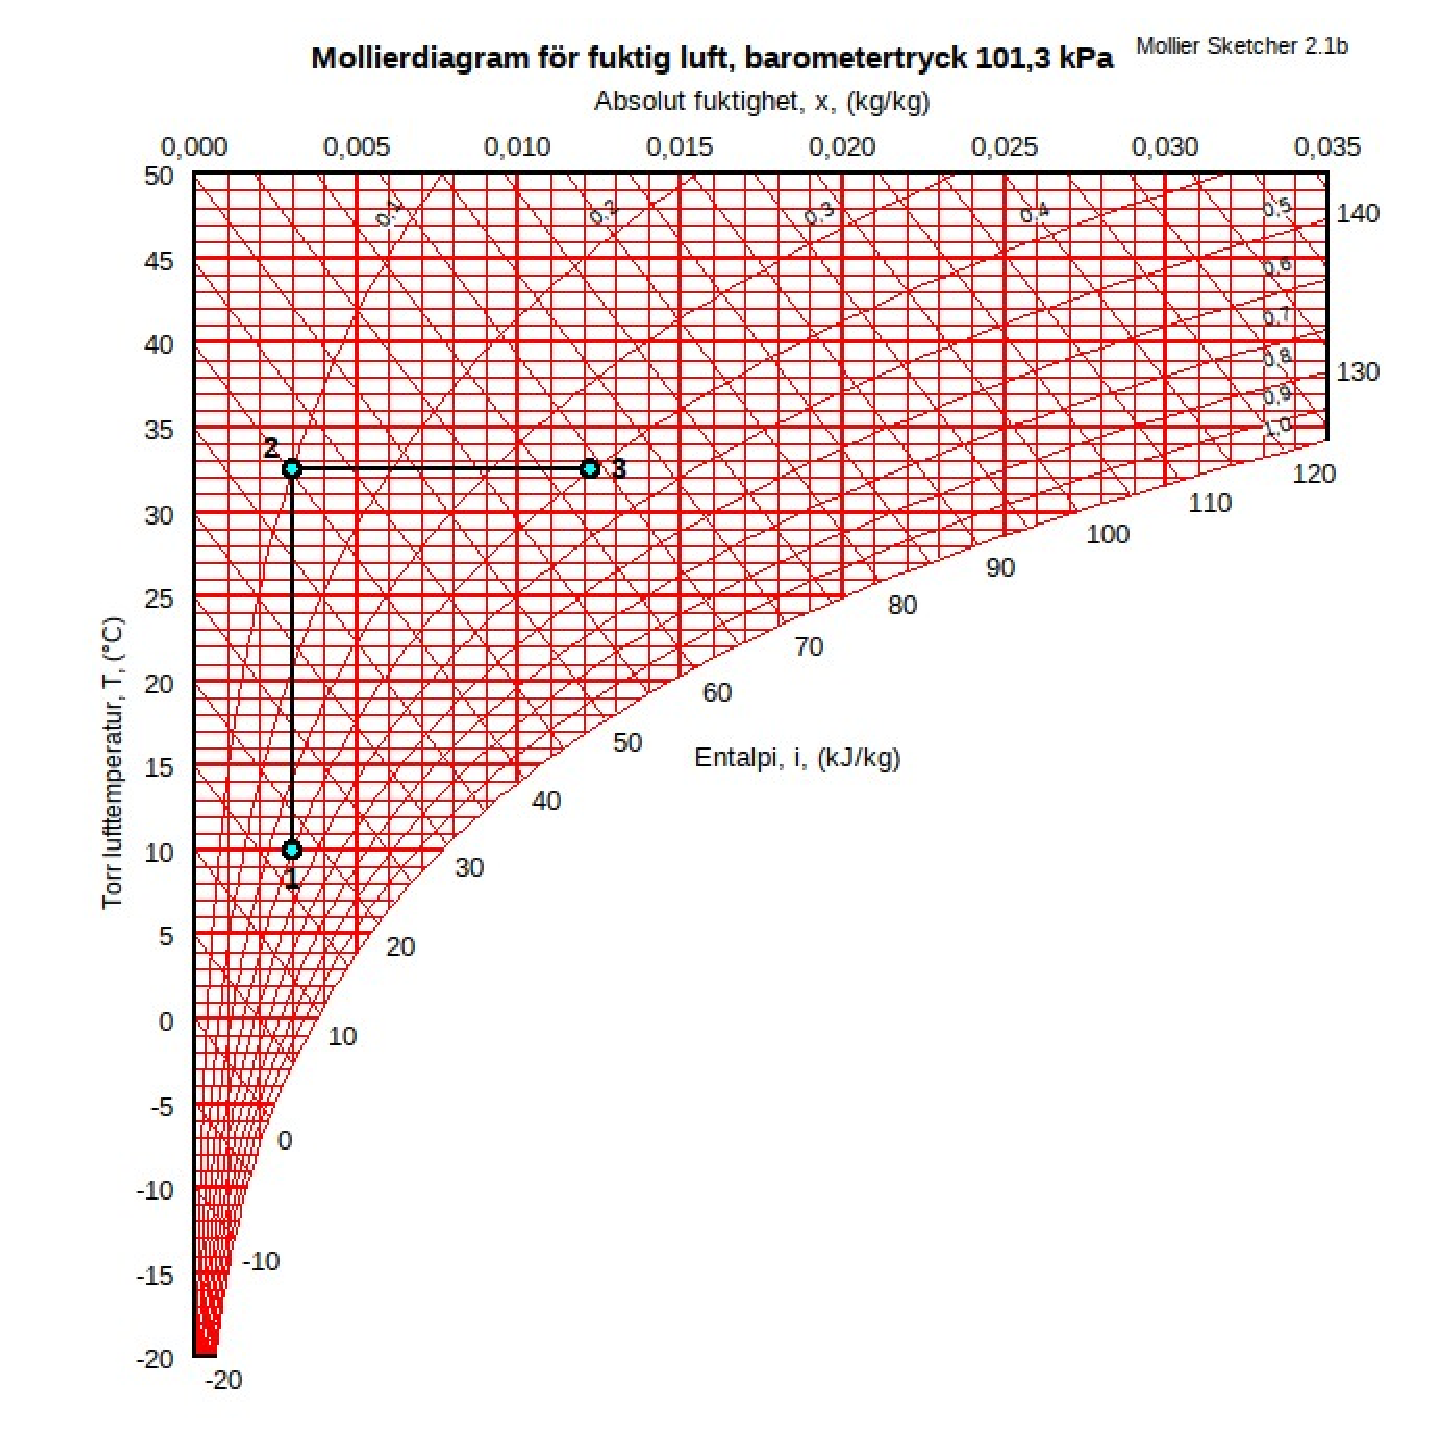
\includegraphics[width=\linewidth]{E20210602.eps}
  \caption{Mollier diagram}
  \label{fig4}
\end{figure}

Vi måste öka vatten halten dvs. kg torr mättad ånga från
3.03 g per kg torrluft till 12.25 g per kg torr luft.
dvs. öka vattenmängden med 12.25-3.03 =  9.22 g per kg torr luft

\end{enumerate}
%\underbrace{}

% \hspace{1em}

%\begin{enumerate}[label=(\alph*)]
%\end{enumerate}

%$$
%  A = 
%  \begin{bmatrix}
%    1 & 0  & 2i\\
%    2i & 0 &  -4\\
%    -i &  0 & -2i\\
%  \end{bmatrix}
%$$

%\begin{flalign*}
%  A = 
%  \begin{bmatrix}
%    1 & 0  & 2i\\
%    2i & 0 &  -4\\
%    -i &  0 & -2i\\
%  \end{bmatrix}
%\end{flalign*}


%\begin{flalign*}
%\psi(x) = \begin{cases} Ae^{ikx}+Be^{-ikx} &\ \  x<-a \\
%                        Ce^{\kappa x}+De^{-\kappa x} &\ \ -a < x < a\\
%						Fe^{ikx} & \ \ x>a
%       \end{cases}
%\end{flalign*}

%\begin{figure}[H]
%  \includegraphics[width=\linewidth]{odd_finite.eps}
%  \caption{$z_0=0.1\pi,0.5\pi, 3\pi,7\pi$}
%  \label{fig4}
%\end{figure}
\end{document}
